\documentclass[a4paper,11pt, titlepage]{article}
\usepackage[T1]{fontenc}
\usepackage[english]{babel}
\usepackage{amsmath}
\usepackage{amsfonts}
\usepackage{color}
\usepackage{graphicx}
\usepackage{subfigure}
\usepackage{epsf}
\usepackage[left=2cm,right=2cm,top=2cm,bottom=2cm]{geometry}
\usepackage{float}
\usepackage{lmodern} 
\usepackage[table]{xcolor}
\usepackage{multirow}
\usepackage{listings} 
\usepackage[justification=centering]{caption}
\usepackage{hyperref}
\usepackage[cc]{titlepic}
\usepackage{fancyhdr}
\usepackage{etoolbox}

%ttfamily

\lstset{% 
language=r, 
basicstyle=\scriptsize, 
keywordstyle=\color{blue}\bfseries, 
commentstyle=\color{black!20!green}, 
stringstyle=\color{red}, 
numbers=left,
numberstyle=\tiny,
frame=\lines
} 

\title{\Huge{Machine learning models for claim prediction in car insurance}}
\author{\Large{Barbara {\sc Gendron-Audebert}}}
\date\today
\titlepic{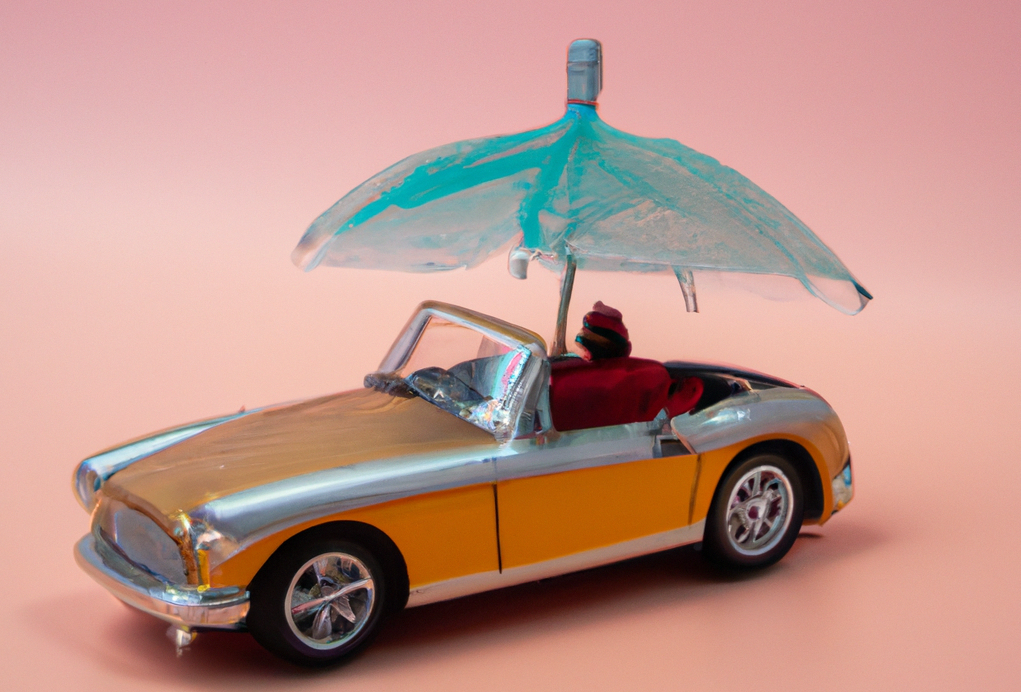
\includegraphics[width=\textwidth]{cover-image.png}}

\patchcmd{\maketitle}
  {\end{titlepage}}
  {\thispagestyle{titlepagestyle}\end{titlepage}}
  {}{}

\fancypagestyle{titlepagestyle}
{
   \fancyhf{}
   \fancyfoot[C]{\emph{A car facing dangers in a hostile planet, protected with an umbrella}, DALL.E generated illustration}
   \renewcommand{\headrulewidth}{0 mm}
}


% --------------------------------------------------------------

\begin{document}
\maketitle
\tableofcontents
\vskip100pt
\section*{Foreword}

This report gives some insights about the use of machine learning techniques in car insurance context. The goal of this work is to leverage data on policyholders related to their driving experience to predict the occurence of a claim. The dataset used to conduct this analysis comes from \href{https://www.kaggle.com/datasets/sagnik1511/car-insurance-data}{this Kaggle page}.\\
\\
In the following sections, we first explore the dataset and describe the related insurance problem in part \ref{data}, before diving in a deeper analysis of the provided features in part \ref{analysis}. In part \ref{models}, one can find insights about the models used to solve this problem, such as a representation of the decision process leading to the model predictions. Finally, part \ref{results} brings a discussion about the provided results, along with some take-aways of this study about car insurance claim prediction.\\
\\
All the technical specifications, the data, all the plots and especially the code (in R) are available in the attached files of the report, and online in \href{https://github.com/B-Gendron/car-insurance-data}{this Git repository}.

\newpage

\section{Data and related insurance problem} \label{data}

\subsection{Dataset description}

This dataset contains exactly 10000 samples, and 19 columns.\\

\noindent The credit score reflect the ability for a policyholder to pay for his debts. The higher the score, the more creditworthy the policyholder is. In car insurance, it is has been observed that this parameter has a significant influence on the insurance rate.\\
{\tt DUIS} refers to DUI, which stands for \textsl{driving under the influence} (whether it be alcohol or drugs).

\subsection{The insurance context}

% -------------------    ANALYSIS    -------------------- % 

\section{Preliminary analysis of the data} \label{analysis}
\subsection{Exploratory data analysis}

In this part I will conduce an exploratory data analysis focusing on the following points:
\begin{itemize}
    \item distribution of variables for numerical ones
    \item distribution of numerical features depending on the {\tt OUTCOME} value
    \item classes distributions depending on the {\tt OUTCOME} value for categorical features
\end{itemize}

\subsubsection{Distribution of variables and classes balance}

\subsubsection{Distribution of numerical features depending on the {\tt OUTCOME} value}

The following figure aims at showing how different is the distribution of a certain numerical feature with respect to the {\tt OUTCOME} value. For this purpose, I used violin plots, which are basically boxplots enhanced by showing the shape of the distribution.

\subsubsection{Classes distributions depending on the {\tt OUTCOME} value for categorical features}

\subsubsection{Dataset summary and completeness of the dataset}

Using the {\tt summary()} R function, we observe that the variables {\tt CREDIT SCORE} and {\tt ANNUAL MILEAGE} respectively have 982 and 957 NA's values. This represents approximately 1\% of the whole data for each variable, that's why we can consider simply delete them. Thus, the remaining dataset contains 8149 rows. 

\section{Brief description of the models used} \label{models}


\section{Analysis of the results and conclusion} \label{results}
\rowcolors{2}{white}{white}
\begin{table}[ht]
    \begin{tabular}[t]{|c|ccccc|}
        \rowcolor{orange!30}
\hline
\textbf{Model} & \textbf{Accuracy} & \textbf{Sensitivity} & \textbf{Specificity} & \textbf{PPV} & \textbf{NPV} \\
\hline
Logistic regression         & \underline{0.8245} & 0.8629 & \underline{0.7334} & \underline{0.8850} & 0.6923 \\
Decision Tree Classifier    & 0.8164          & 0.8534 & 0.7252 & 0.8844 & 0.6675 \\
Random Forest Classifier    & \underline{0.8245} & \underline{0.8719} & 0.7206 & 0.8725 & 0.7197 \\
XGBoost                     & 0.8164          & 0.8844 & 0.6675 & 0.8534 & \underline{0.7252} \\
\hline
    \end{tabular}
\centering
\caption{A sum-up table of the classification metrics for each model. PPV stands for Predicted Positive Values and NPV stands for Negative Predicted Values.}
\label{metrics}
\end{table}%

\appendix

\section{Appendix}

\rowcolors{2}{gray!20}{white}

\begin{table}[ht]
    \begin{tabular}[t]{|lcc|}
        \rowcolor{orange!30}
\hline
\textbf{Variable}           & \textbf{Type}      & \textbf{Value ranges (if meaningful)}     \\
\hline
VEHICLE OWNERSHIP   & Binary    & 0 or 1                     \\
MARRIED             & Binary    & 0 or 1                     \\
CHILDREN            & Binary    & 0 or 1                    \\
OUTCOME             & Binary    & 0 or 1                     \\
AGE                 & Category    & 16-25, 26-39, 40-64, 65+      \\
GENDER              & Category    & female, male                  \\
RACE                & Category    & majority, minority            \\
DRIVING EXPERIENCE  & Category    & 0-9y, 10-19y, 20-29y, 30y+     \\
EDUCATION           & Category    & high school, none, university \\
INCOME              & Category    & middle class, poverty, upper class, working class \\
VEHICLE TYPE        & Category    & sedan, sports car             \\
VEHICLE YEAR        & Category    & after 2015, before 2015       \\
CREDIT SCORE        & Float     & From 0.0534 to 0.9608       \\
ID                  & Integer   & --                \\
POSTAL CODE         & Integer   & --             \\ 
ANNUAL MILEAGE      & Integer   & From 2000 to 22000               \\ 

SPEEDING VIOLATIONS & Integer   & From 0 to 22                   \\
DUIS                & Integer   & From 0 to 6                      \\ 
PAST ACCIDENTS      & Integer   & From 0 to 15                    \\  

\hline
    \end{tabular}
\centering
\caption{A short description of the covariates, along with some insights about categorical variables.}
\label{data-description}
\end{table}%

\begin{figure}[!h]
    \centering
    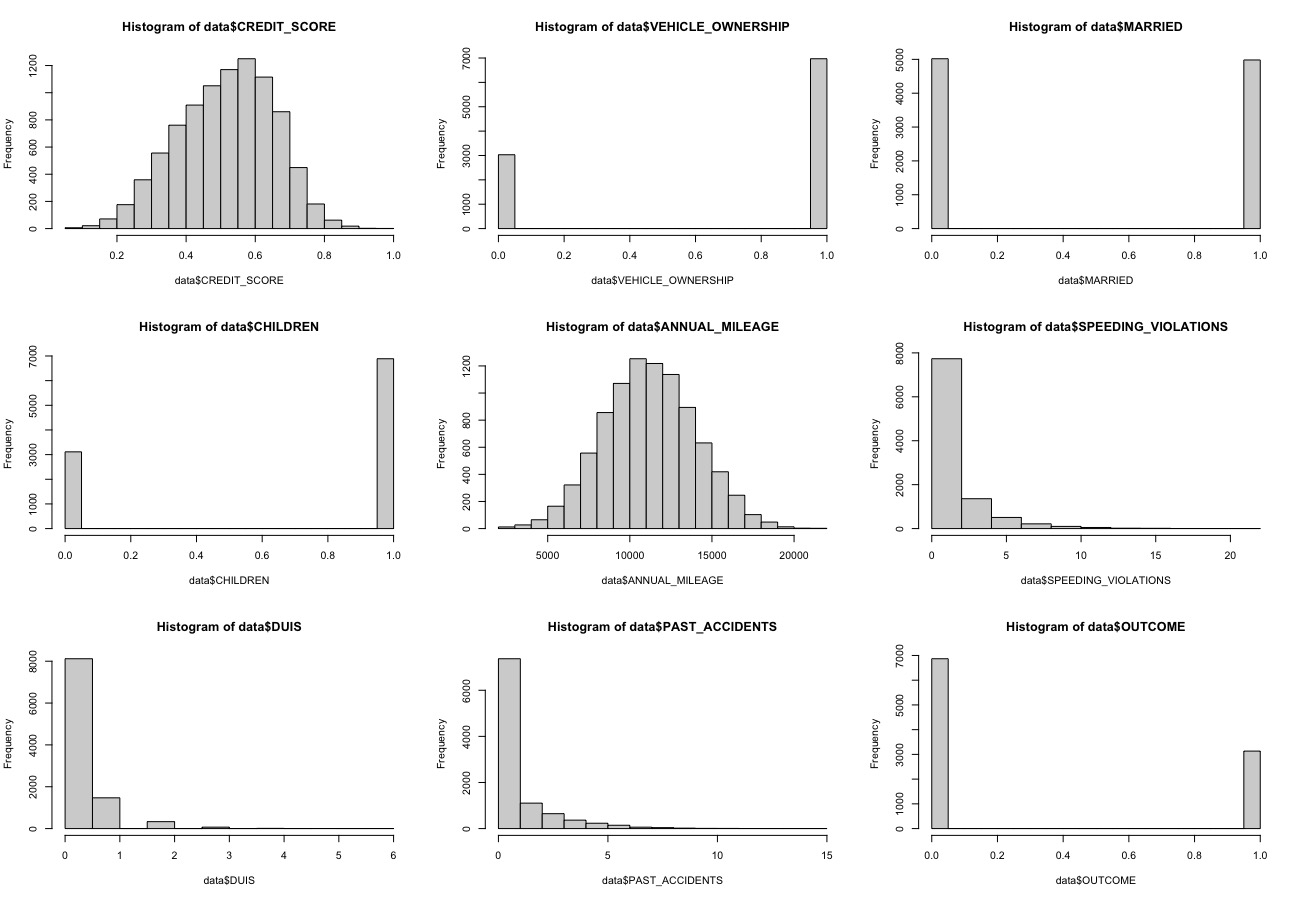
\includegraphics[scale=0.35]{eda.jpeg}
    \caption{Histograms of the numerical variables.}
    \label{fig:histograms}
\end{figure}


\begin{figure}[!h]
    \centering
    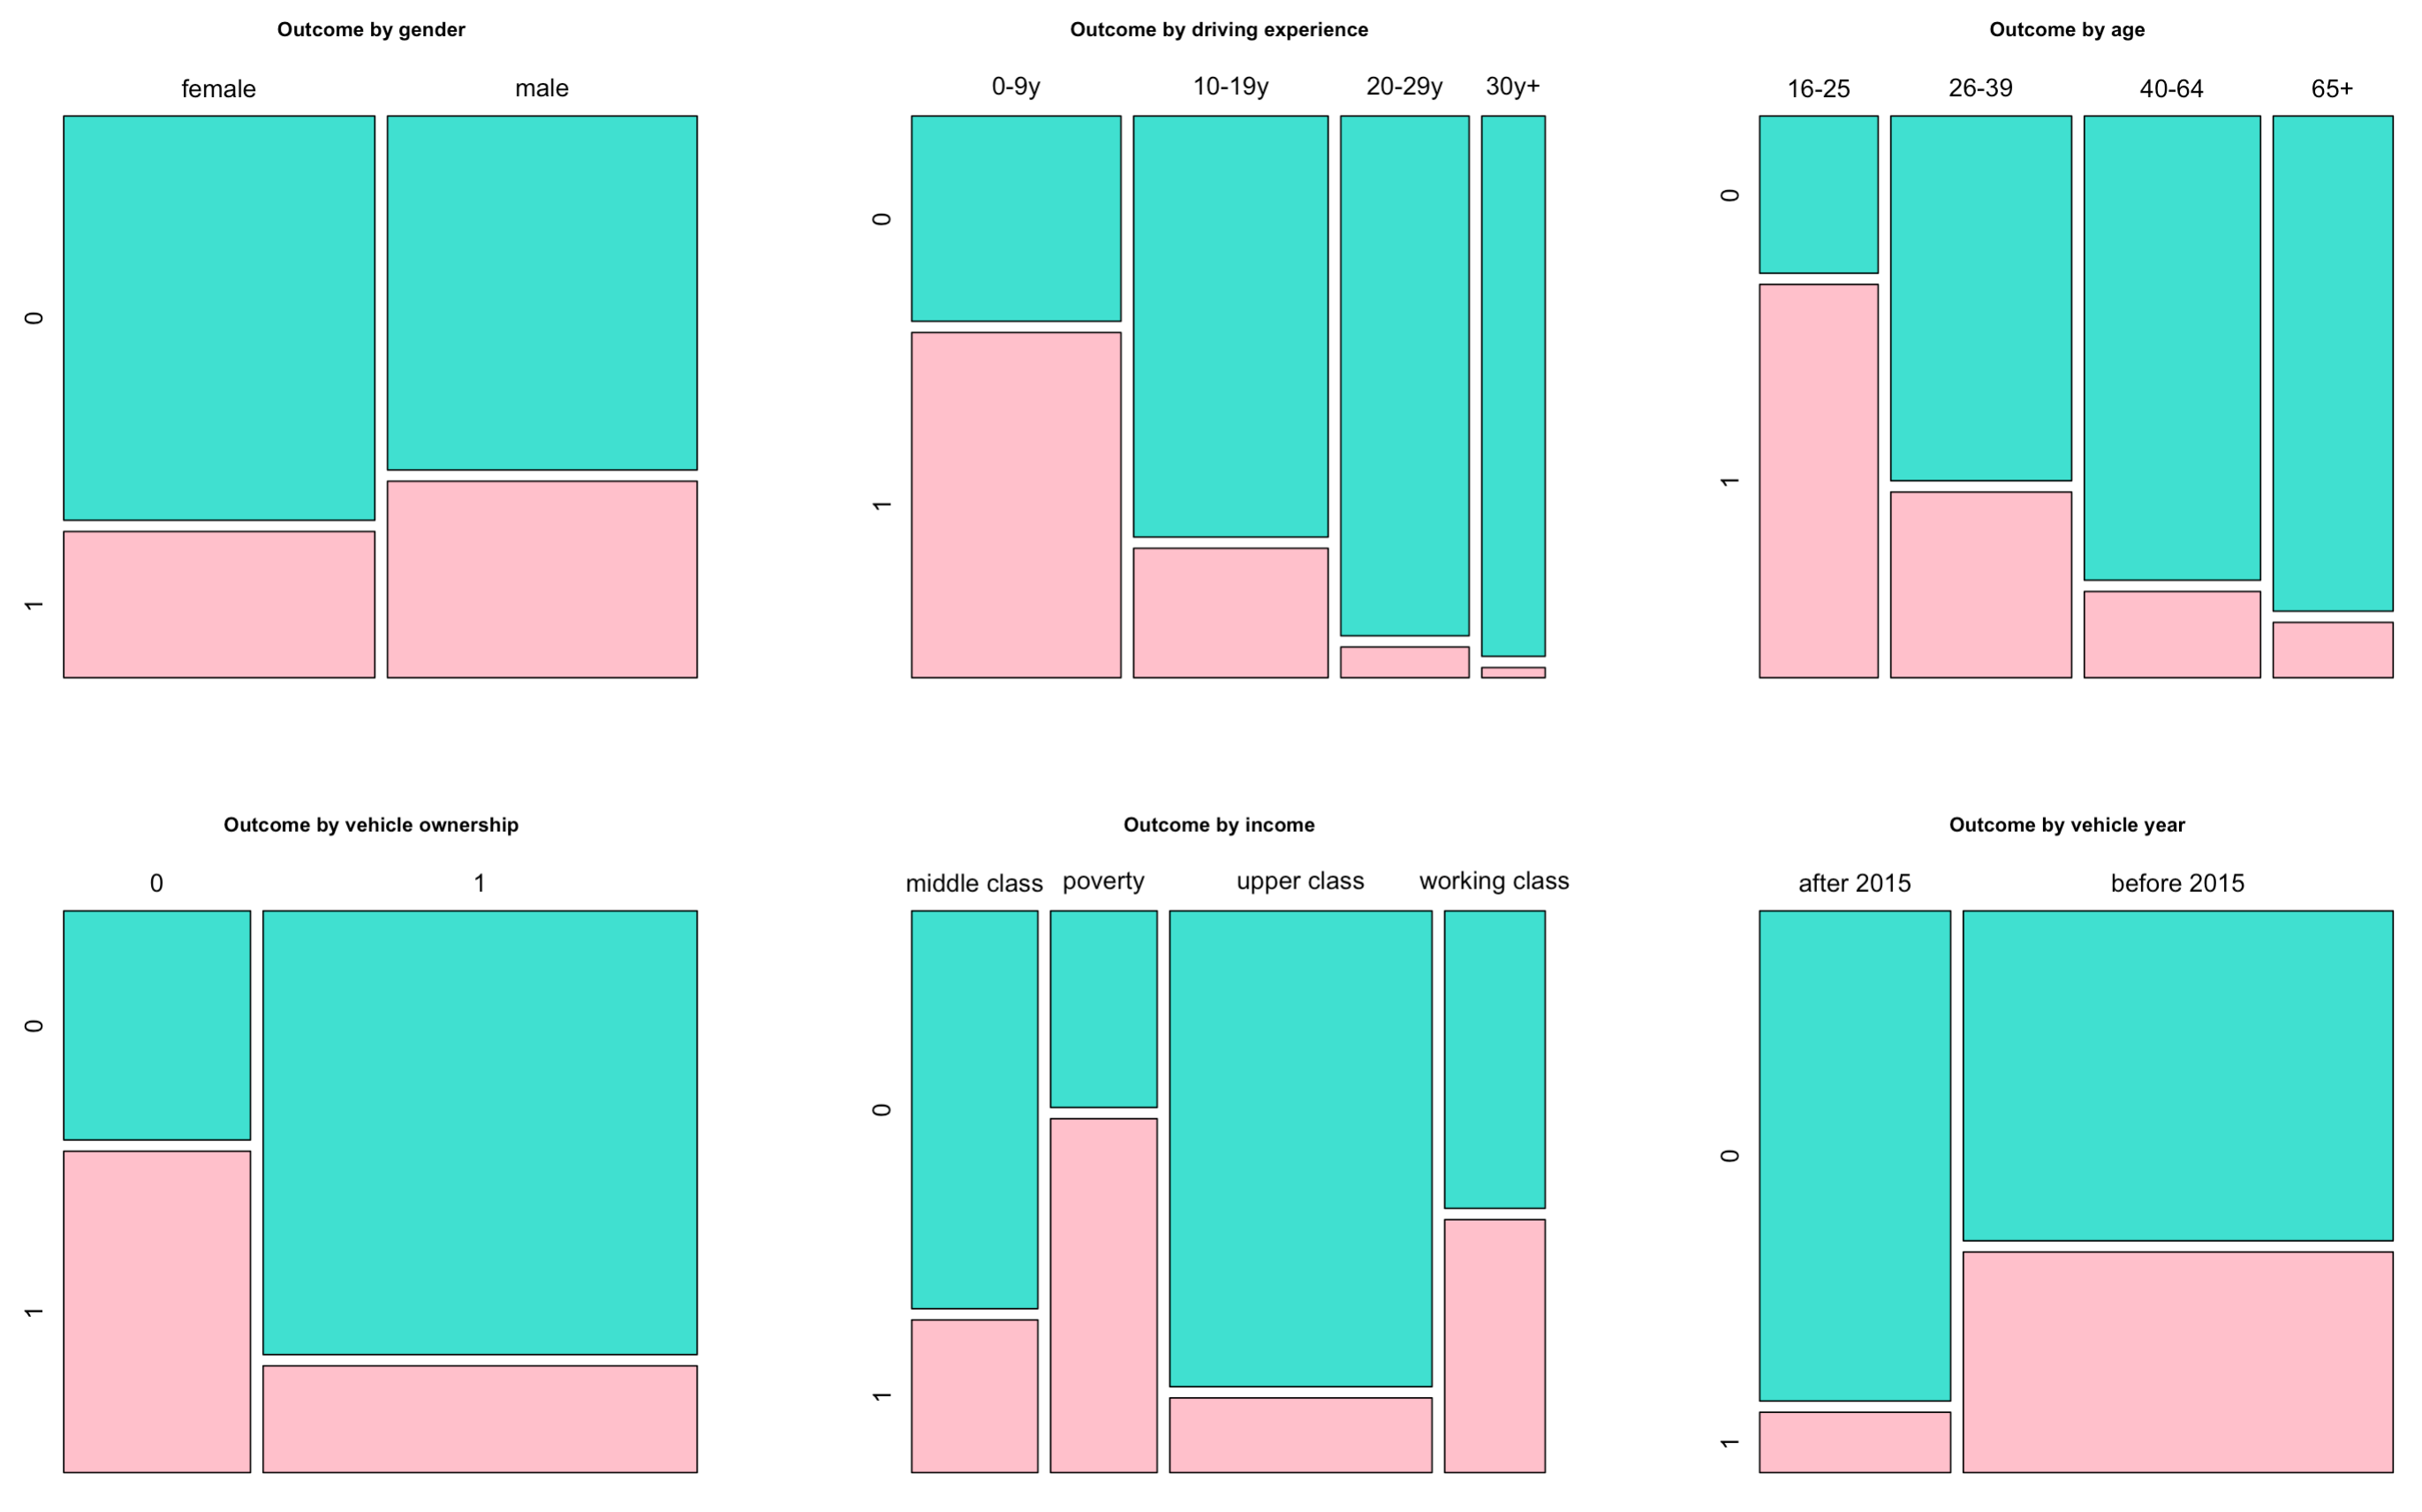
\includegraphics[scale=0.3]{eda-report.png}
    \caption{Value counts of categorical features with respect to the {\tt OUTCOME} value.}
    \label{fig:categorical-counts}
\end{figure}

\end{document}